\documentclass{vldb}

\usepackage{graphicx}
\usepackage{listings}
\usepackage{subcaption}
\usepackage{caption}
\usepackage{hyperref}
\lstset{
  language=C,
  basicstyle=\ttfamily\scriptsize,
  tabsize=2,                    % sets default tabsize to 2 spaces
%  columns=flexible,
  xleftmargin=18pt,
  xrightmargin=1em,
  numbers=left,
  numberstyle=\scriptsize,
  numbersep=1em,
  showstringspaces=false,
  alsoletter={-},
	morekeywords={todo}, %FIXIT
	otherkeywords={TD},  %FIXIT
  captionpos=b,
  escapeinside={@}{@},
  commentstyle=\color{gray},
}


\begin{document}

\title{Incremental Memory Cost Model for MonetDB}

\author{Pavlos Katsogridakis, Ying Zhang, Martin Kersten}

\maketitle

\begin{abstract}
Estimating the memory footprint of a query is an important
feature for a database system. It can answer the question whether
a query will fit in memory, and also gives the compiler the opportunity
to perform a lot of optimizations.
In this document we present Malcom (Mal ALgebra COst Model), a memory footprint
estimator, that incrementally builds a memory cost model for MAL instructions,
based on previous query executions. We evaluated our system using the tpch
benchmark suite, and a real world air traffic dataset.
\end{abstract}

\section{Introduction}
\label{Introduction}
Since its inception, database designers have keenly looked at the opportunities to use large,
distributed processing platforms. Cluster-based products are readily available \cite{},
but are often limited to a few tens of compute nodes and call for a strong engineering
to avoid hardware bottlenecks, such as in Exadata \cite{}, SQL PWD \cite{}, IBM Blu \cite{} and ....

A plethora of research activities have shows that in all but the simplest cases,
achieving a good performance is at least very hard. Especially when the query
involves joins spread over multiple compute nodes and require an expensive data exchange.

The predominant way out, taken in NoSQL systems  \cite{Casandra,Impala}
is to address part of the problem space by focusing on select-aggregate queries.
This focus on part of the problem space for distributed query processing has
been shown pivotal to support big-data analytics in many real-world circumstances,
as shown by the widespread use of Spark \cite{},
which is widely used nowadays to encode distributed applications.
The basic abstraction in Spark is a Resilient Distributed Dataset (RDD),
which represents an immutable, partitioned collection of elements that can be
operated on in parallel using operators, such as map, filter, persist and aggregates.
Moreover, the RDD is the basic component to exchange between
operators, threads, cores and machines.
In essence, an RDD can be seen as a relational table used for interoperability,
an approach that can be traced back to Microsoft's ODE \cite{} used for decades
to exchange data between DBMS and applications. Similar functional abstractions
can nowadays be found in R's Dataframes \cite{} and Python Pandas\cite{}.

%explain resident/resilient, the former tells it can be re-constructed upon need.

Although in most cases, it is easier to scale-up for improved response time,
partitioning a database to benefit from the low price tag, better use of parallel IO,
or resource limitations of smaller machines is still worth considering.
Distributed database management systems have followed the same route \cite{distributed DB}.
However, the major hurdle that has blocked progress for decades is the insurmountable task
to create an optimizer to derived an optimal plan \cite{}.

In this paper we take a fresh look at optimizing query processing in the context
of where intermediates in a query plan are fully materialized before passing on
towards the next operator. This model fits the Spark programming model,
but also the query execution model underlying MonetDB.
Resilient intermediates provides new avenue for query optimization and
scheduling as it underlying computation model is based on
materialization of all intermediate steps.

The main contributions of this paper are
\begin{itemize}
	\item we develop a simulator to predict size and processing bounds for queries based on resident intermediates.
	\item We provide a novel optimizer to minimize memory footprint and processing time
	\item We demonstrate the approach is robust against varying data distributions.
	\item We demonstrate the quality of our approach using an extensive evaluation against TPC-H and real-world databases.
	\item ...
\end{itemize}

The approach taken differs from traditional cost-based optimizers by sampling
the state of actual execution of primitive operations.
For, after each query step we have precise knowledge of the resources claimed.
This information can be harvested and to predict future operations of similar nature.
The rational stems from the common knowledge that any database application
environment has a limited number of 'business transactions' or 'BI templates'
where only some parameters are changed with each call.
This knowledge has been used in the past to drive development of DBA
wizards \cite{microsoft} for index selection and self-tuning optimizers
\cite{IBM} to avoid expensive join paths.

Outline of paper. Section \ref{Background} provides a short introduction
to the MonetDB architecture and the projects involved.

\subsection{Use Cases}
\begin{enumerate}
  \item Prediction of the memory footprint
  \item Instruction ordering by the compiler
  \item Parallelism level
  \item Join dictionary build
\end{enumerate}

\section{Background}
\label{Background}
In this section we summarize the salient features of resilient intermediates
for query processing., the leading open-source column store and the envisioned
system ExaNest, an exascale HPC platform for data-intensive computing.

\subsection{A Column Store}
%Recap some MonetDB stuff on how queries are compiled.
MonetDB is a widely used column store that internally uses resident
intermediates to break up query processing in well identified steps.
The query plan is broken up into independent steps, glued together into a
dataflow dependency graph. The dataflow graph is greedily consumed by the
database kernel assigning a single core to a single operation.
The resource pressure is kept at a minimal to trim down the degree of parallel
processing when the main resource, RAM, is heavily used.
The system can be instructed to produce an event record for each completed instruction.
This provides a.o. insight into the input/output sizes and timing.

\subsection{Distributed Query Optimizers}
% summarize
The predominant scheme to scale out database processing is to break the base
tables into independent partitions using either a hash-key or ranges.
The partitioning scheme can be used to orchestrate distributed processing
in an optimal way most of the time.

Apache Spark CBO\footnote{\url{https://databricks.com/blog/2017/08/31/cost-based-optimizer-in-apache-spark-2-2.html}}: add some description


\section{Micro Models}
With an abundance of events we can start to derive models for each of the instructions.
A micro model is derived that can be used later for ease of simulation
alternative execution plans. We study them based on similar properties.

\subsection{Arithmetic Operations}
The operations can be grouped by complexity to predict the outcome of a hypothetical operation.
The first group includes the {\em batcalc} operations.
They all obey the following structure:
\begin{verbatim}
  res:bat[:lng]:= batcalc.==( l:bat[:lng],r:bat[:lng])
  res:bat[:lng]:= batcalc.==( l:bat[:lng],r::lng)
  res:bat[:lng]:= batcalc.==( l:lng,r:bat[:lng])
  res:bat[:lng]:= batcalc.==( l:lng,r:lng)

\end{verbatim}
The argument is either scalar or a reference to a column.
However, in all cases the number of result tuples can be looked up from the argument events.
The processing time depends mostly on the type's footprint and the influence of concurrent activity.


\subsection{Limit Operations}
Limit and sample operators(firstn, and sample? in MAL) are also trivial,
we just output the minimum of the argumens size and the limit size.


\subsection{Aggregate Operations}
This category includes operations like sum, avg, min, max, single, dec\_round
The count of the result is obviously one.

\subsection{Select Operator}
\subsubsection{Range Selects}
To predict the size of a range select, we used the kNN algorithm,
using k=5, to find the 5 closest selects to the one we want to predict,
considering the lower and higher bounds as distance metrics.
When we are facing a one bound select ($<$,$>$ etc) we use the
dataset statistics to fill the other bound (e.g in case of $<$ we want the column min).
\subsubsection{Point Selects}
Nothing special, we try to find the most similar point....

\subsubsection{Like Selects}
Future work :P

\subsubsection{Subsequent Selects}
%TODO make it more general
In case of intermediate select instructions, the ranges are not adequate to
make an accurate prediction, because the argument size may vary based on the
previous selects. To overcomes this we incorporated the estimations of the
previous intructions, to build a graph that relates each variable to a size
estimation. This way we cal also use the argument estimation to predict the
size of the select result. The code for selection prediction is shown at
Figure\ref{sel:code}. In real life it is very common to find correlated columns,
in which the first selection may affect non-linearly the second.
In our design we do not handle such cases(Future work).

\begin{figure}[t]
\begin{lstlisting}[frame=single]
  def div(i1, i2):
    return (i1.hi-i1.lo) / (i2.hi-i2.lo)

  def extrapolate(traini, testi):
      traini.cnt*div(testi,traini)*testi.approx_arg_cnt/traini.argcnt

  def predict(testi, traind, approxG):
    knn5 = traind.knn(testi,5)
    return sum([i.extrapolate(testi) for i in knn5]) / len(knn5)
\end{lstlisting}
  \caption{Code snippet for making predictions for range selects}
  \label{sel:code}
\end{figure}


\subsection{Join}
Nothing special yet
(Run a kNN to the previous joins that operate on the same two columns if possible,
and find the ones closest based on the argument sizes)

\subsection{Grouping Operations}
The groupby signature is:
\begin{verbatim}
  (bat[:oid], bat[:oid], bat[:X]) := group.groupdone(bat[:X]);
\end{verbatim}
The first return value is the ids of the grouped column, the second is
the ids of the discinct values of the column(the third what ??). To predict
the size of the return variables, we use the ground statistics of the column
(size, count, discinct values).

Subgroupdone has a similar signature to groupdone, but it operates on intermmediate
variables, where we do not have the column information. In this case, we run a
kNN based on the argument sizes.

Orderby is translated into sort in MAL.
\begin{verbatim}
(bat[:X],bat[:oid],bat[:oid]) := algebra.sort(bat[:X], bat[:oid], bat[:oid], bit, bit)
\end{verbatim}
The size of each return value is exactly the same as the corresponding argument size.

\subsection{Set instructions}
We do not have any relevant information to do an accurate guess for the
set instructions, so we output the worst case of the result.
$$ intersect(A,B) ~= min(A,B)$$
$$ merge(A,B) ~= A+B $$
$$ diff(A,B) ~= A $$
% diff,union,intersect

\subsection{Load instructions}
\subsubsection{bind}
Bind instruction loads(or memory maps) a column into memory,
thus the result size is the size of the column.
\subsubsection{bind\_idxbat, tid}
Tid and bind\_idxbat do not produce any memory overhead

\subsection{Special cases}
\subsubsection{String sililarity}
In predicting a selection of a string column,
we used the levenshtein distance as a metric...
\subsubsection{Projection returning str}
In some weird cases, the projection instruction
returns str(copies from heap) instead of ids,
which makes hard to predict. In this case, we run a kNN
based on the type and argument distance, to find a similar
instruction use this to find the output size.

\section{Experiments}
\subsection{Tpch SF10}
% To evaluate our memory footpring estimator mechanism we kept each
As a training set for each query, we randomized every selection point and range,
and produced 200 random versions of the query. As a test set we used the original
query.

In query 19 we observe a misprediction of 70\%. The reason this happens, is that
the MAL algebra of this specific query consists of a lot of merge instructions,
for which we output the sum of the two arguments, which in case of merging similar
variables can lead to an almost 2$\times$ overestimation.
This is the basic reason for the large error observed.
\begin{verbatim}
culprit:
C_187 := algebra.thetaselect(X_178, "DELIVER IN PERSON", "==");                                                                                                                                                                                                                    |
X_191 := bat.mergecand(C_187, C_187);                                                                                                                                                                                                                                              |
X_194 := bat.mergecand(X_191, C_187);
\end{verbatim}

The second most deviant query is 16. The dominant reason why there is an 20\%
error is the misprediction of the join instruction(our approach is kNN based).

\begin{figure}[!htb]
  \centering
  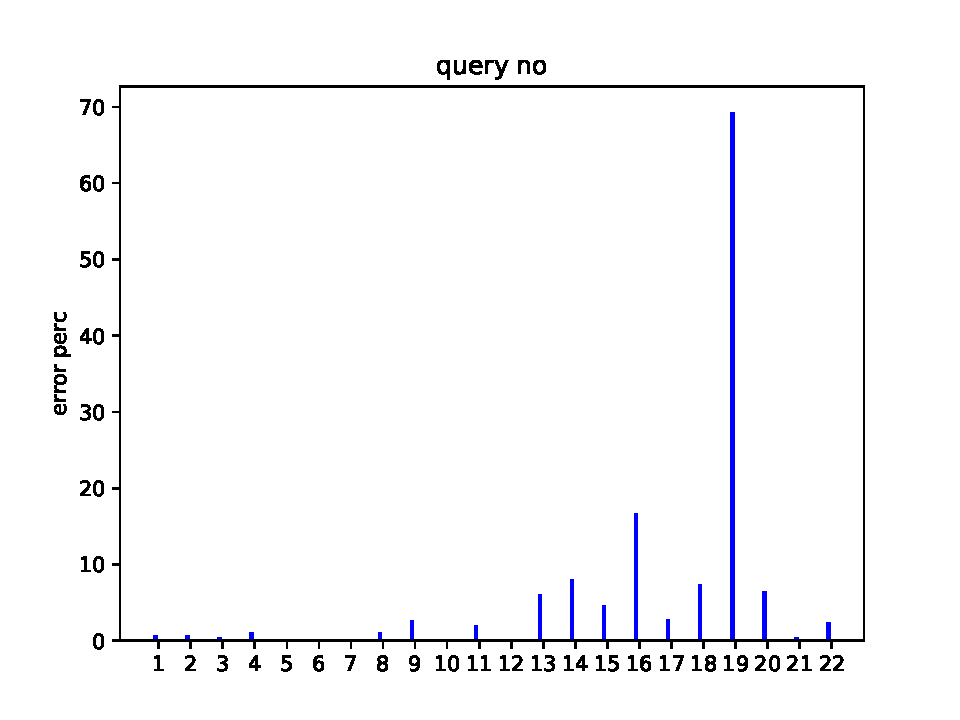
\includegraphics[scale=0.7]{figs/tpch10/mem_error_1-23.pdf}
  \caption{Queries 1-22 memory footprint error}
  \label{fig:tpch10m}
\end{figure}

\subsection{Airtraffic Queries}
%TODO some info about airtraffic...
As a training set for each query, we used 1000 versions of the
same query, randomized on the selection values. As a test set we used the original
query.
\subsubsection{Q04}
Query 4 (Figure \ref{sel:sql4}) selects all flights that have a departure delay greater than 15 minutes.
The training queries are randomized based on the DepDelay bound.
From the prediction perspective, this selection is interesting because
departure delay does not follow a uniform distribution(more like a normal),
thus is more challenging to accurately predict.
Figures  \ref{fig:sel04}, \ref{fig:mem04} show the error percentage for the
selection, and the whole query respectively. The x axis is the number of queries
used as a training set, and the y axis the error \%. The initial selection error
for is 500\%, but as we insert more instructions to the dictionary we get closer
to the initial range, and we are able to make an accurate prediction. After the
first 400 instructions, the error drops to (...)\%.
The per query memory error follows a similar pattern,
but the error is smaller because select instructions represent a relatively
small proportion of the overall query memory usage.

\begin{figure}[t]
\begin{lstlisting}
SELECT "DayOfWeek", COUNT(*) AS "Flights"
FROM ontime
WHERE "DepDelay" > 15
GROUP BY "DayOfWeek"
ORDER BY "DayOfWeek";
\end{lstlisting}
  \caption{Query 4}
  \label{sel:sql4}
\end{figure}


\begin{figure}[!htb]
  \begin{subfigure}[t]{0.5\textwidth}
    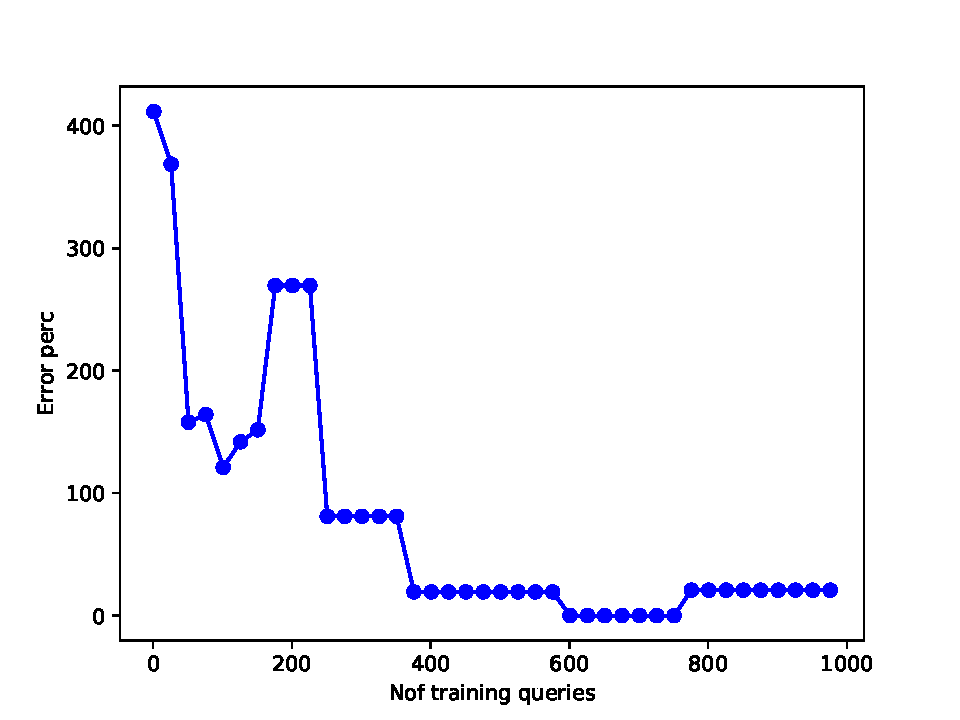
\includegraphics[scale=0.4]{figs/airtraffic/airtraffic_sel04_error.pdf}
    \caption{Query 04 select error}
    \label{fig:sel04}
  \end{subfigure}
  \begin{subfigure}[t]{0.5\textwidth}
    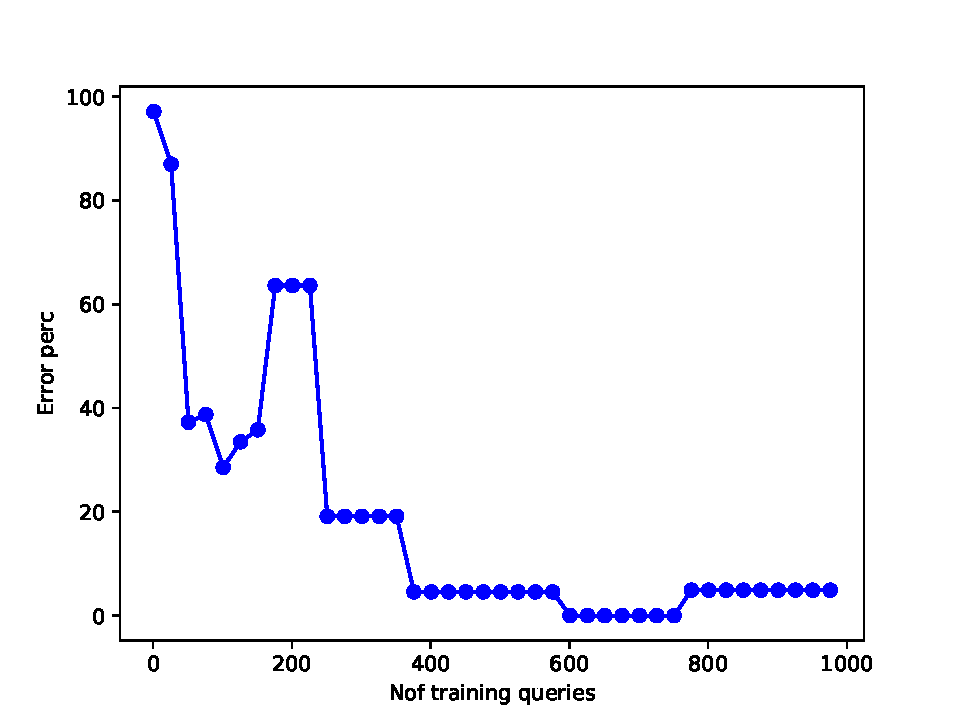
\includegraphics[scale=0.4]{figs/airtraffic/airtraffic_q04_memerror.pdf}
    \caption{Query 04 memory footprint}
    \label{fig:mem04}
   \end{subfigure}
\end{figure}

\subsubsection{Q09}

Query 9(Figure \ref{sel:sql09}) selects all flights on a specific date
for which the departure and the arrival delay are greater than 15 minutes.
The memory error(Figure \ref{fig:sel09}) is very small,
due to the very high selectivity of the query,
whereas the selection error(Figure \ref{fig:mem09}) seems to fluctuate a lot
betwwn 20 and 40\%. The reason we believe this is happening is that all three columns
(depdelay, arrdelay, date) are strongly correlated, making it very hard
for the prediction algorithm to converge.

\begin{figure}[!htb]
\begin{lstlisting}[frame=single]
WITH t1 AS (
    SELECT "Origin","CRSDepTime","DepDelay","Dest","ArrDelay","CRSArrTime"
    FROM ontime
    WHERE "DepDelay" > 15 AND "ArrDelay" > 15
      AND "Month" = 3 AND "DayofMonth" = 24 AND "Year" = 2013
)
SELECT t1."Origin" AS "Airport1",
  CAST(AVG(t1."DepDelay") AS DECIMAL(8,2)) AS "AVGDepDelay",
  CAST(AVG(t1."ArrDelay") AS DECIMAL(8,2)) AS "AVGArrDelay", t2."Origin" AS "Airport2",
  CAST(AVG(t2."DepDelay") AS DECIMAL(8,2)) AS "AVGDepDelay2",
  CAST(AVG(t2."ArrDelay") AS DECIMAL(8,2)) AS "AVGArrDelay2", t2."Dest" AS "Airport3"
FROM t1, t1 AS t2
WHERE t1."Dest" = t2."Origin" AND t1."CRSArrTime" < t2."CRSDepTime"
GROUP BY t1."Origin", t2."Origin", t2."Dest"
ORDER BY "AVGDepDelay" DESC,"AVGArrDelay" DESC,"AVGDepDelay2" DESC,"AVGArrDelay2" DESC
\end{lstlisting}
  \caption{Query 09}
  \label{sel:sql09}
\end{figure}

\begin{figure}[!htb]
  \begin{subfigure}[t]{0.5\textwidth}
    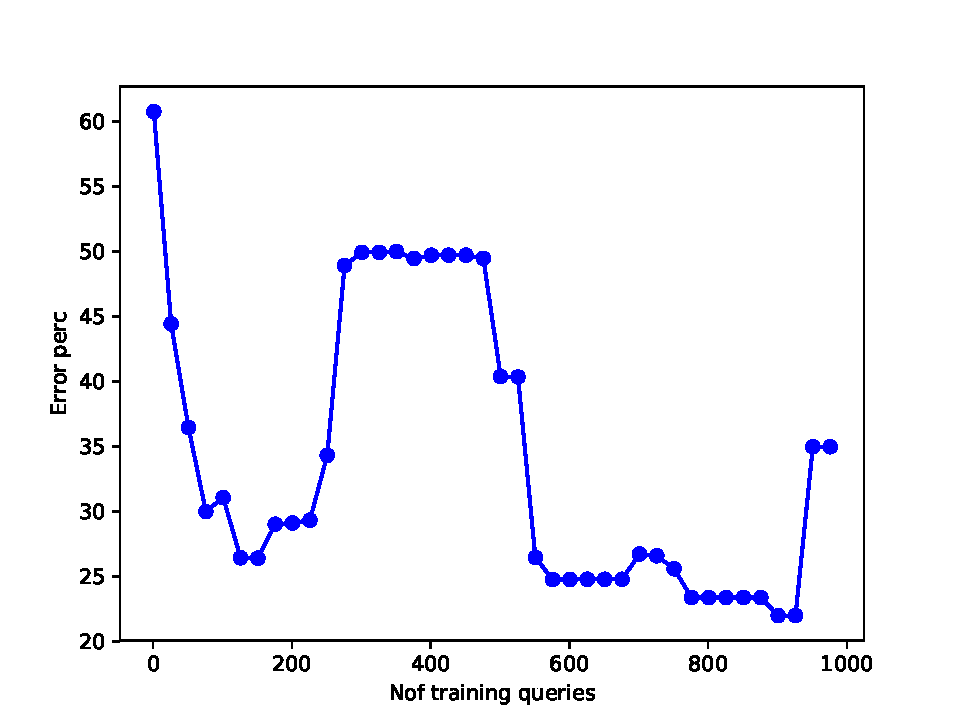
\includegraphics[scale=0.4]{figs/airtraffic/airtraffic_sel09_error.pdf}
    \caption{Query 09 select error}
    \label{fig:sel09}
  \end{subfigure}
  \begin{subfigure}[t]{0.5\textwidth}
    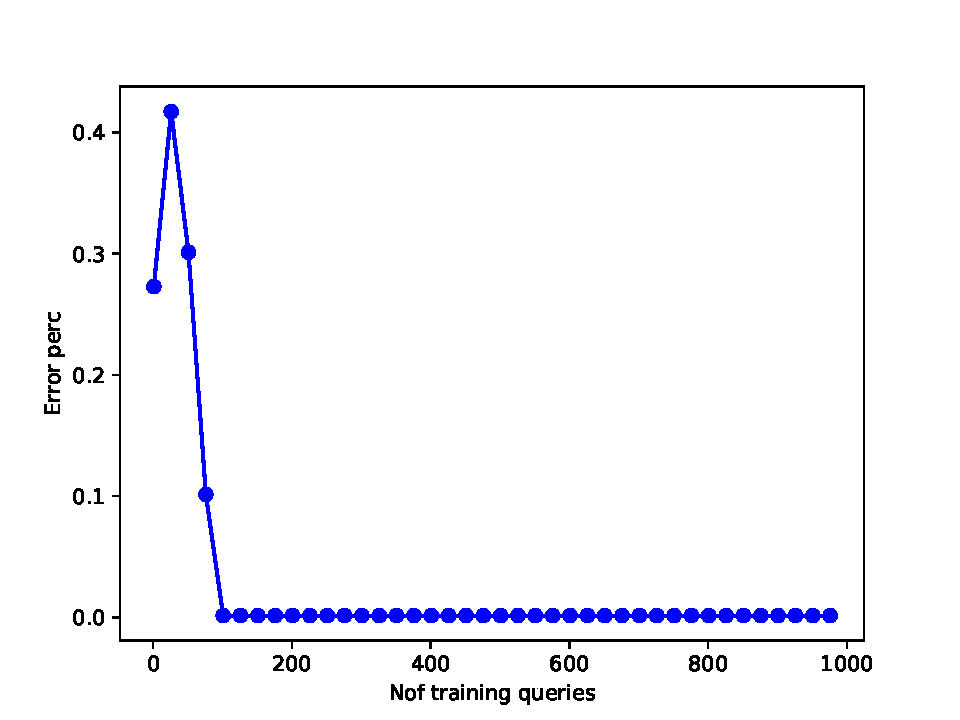
\includegraphics[scale=0.4]{figs/airtraffic/airtraffic_q09_memerror.pdf}
    \caption{Query 09 memory footprint}
    \label{fig:mem09}
   \end{subfigure}
\end{figure}

\subsubsection{Q10}

Query 10(Figure \ref{sel:sql10}) contains two point selections,
regarding the origin and the destination of the flight.


\begin{figure}[htb!]
\begin{lstlisting}[frame=single]
ITH t1 AS ( -- flights to ORD
    SELECT "Origin" AS ap, COUNT(*) AS cnt_in
    FROM ontime
    WHERE "Dest" = 'ORD'
    GROUP BY "Origin"
),
t2 AS ( -- flights from ORD
    SELECT "Dest" AS ap, COUNT(*) AS cnt_out
    FROM ontime
    WHERE "Origin" = 'ORD'
    GROUP BY "Dest"
),
t3 AS ( -- merge t1, t2 into one table
    SELECT t1.ap AS ap1, t1.cnt_in, t2.ap AS ap2, t2.cnt_out
    FROM t1 FULL OUTER JOIN t2 ON (t1.ap = t2.ap))
SELECT CASE WHEN ap1 IS NULL THEN ap2 ELSE ap1 END AS "Airport",
       cnt_in AS "InboundFlights", cnt_out AS "OutboundFlights"
FROM t3;
\end{lstlisting}
  \caption{Query 10}
  \label{sel:sql10}
\end{figure}

\begin{figure}[htb!]
  \begin{subfigure}[t]{0.5\textwidth}
    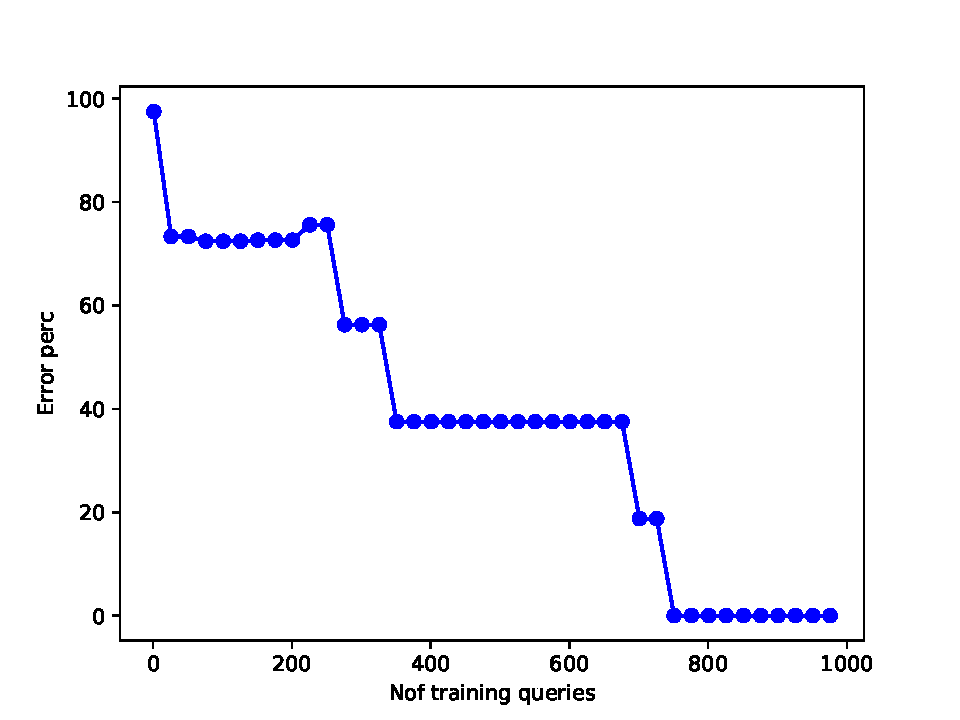
\includegraphics[scale=0.4]{figs/airtraffic/airtraffic_sel10_error.pdf}
    \caption{Query 10 select error}
    \label{fig:sel10}
  \end{subfigure}
  \begin{subfigure}[t]{0.5\textwidth}
    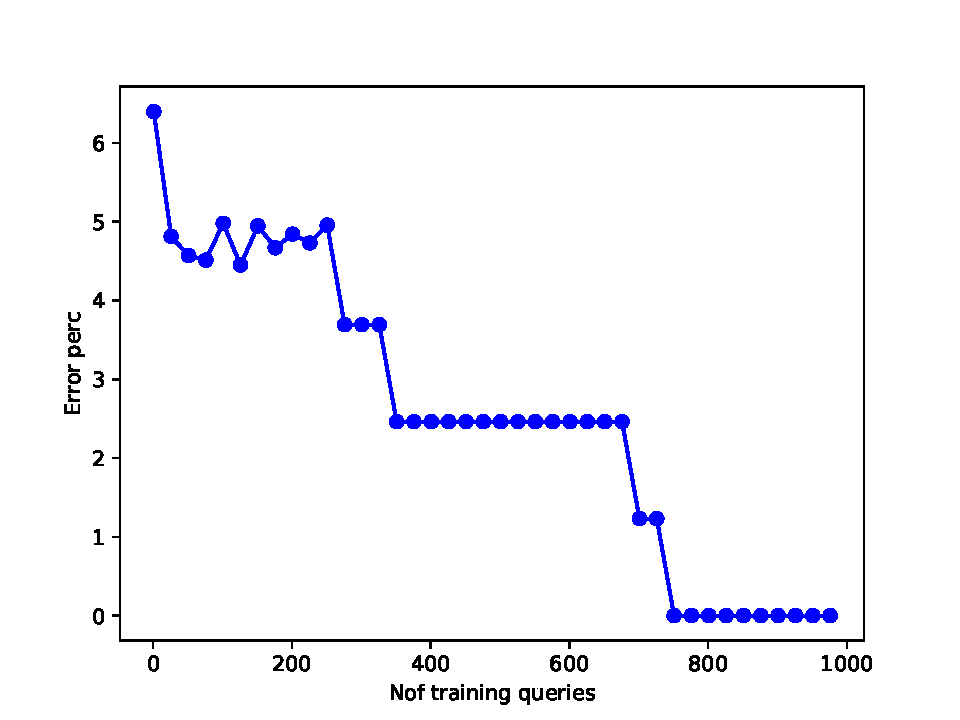
\includegraphics[scale=0.4]{figs/airtraffic/airtraffic_q10_memerror.pdf}
    \caption{Query 10 memory footprint}
    \label{fig:mem10}
   \end{subfigure}
\end{figure}


\subsubsection{Q11}

\begin{figure}[htb!]
\begin{lstlisting}[frame=single]
WITH t1 AS ( -- #flights per route before 9/11
    SELECT SQL_MIN("Origin", "Dest") || ' <-> ' ||
           SQL_MAX("Origin", "Dest") AS route,
           COUNT(*) AS cnt_before
    FROM ontime
    WHERE '2010-09-11' < "FlightDate" AND "FlightDate" < '2011-09-11'
    GROUP BY route
),
t2 AS ( -- #flights per route after 8/11
    SELECT SQL_MIN("Origin", "Dest") || ' <-> ' ||
           SQL_MAX("Origin", "Dest") AS route,
           COUNT(*) AS cnt_after
    FROM ontime
    WHERE '2011-09-11' <= "FlightDate" AND "FlightDate" < '2012-09-11'
    GROUP BY route
),
t3 AS ( -- merge t1, t2 into one table
    SELECT t1.route AS route1, t1.cnt_before, t2.route AS route2, t2.cnt_after
    FROM t1 FULL OUTER JOIN t2 ON (t1.route = t2.route)
)
SELECT CASE WHEN route1 IS NULL THEN route2 ELSE route1 END AS "Route",
       cnt_before AS "FlightsBefore", cnt_after AS "FlightsAfter"
FROM t3;
\end{lstlisting}
  \caption{Query 11}
  \label{sel:sql11}
\end{figure}

\begin{figure}[htb!]
 \begin{subfigure}[t]{0.5\textwidth}
   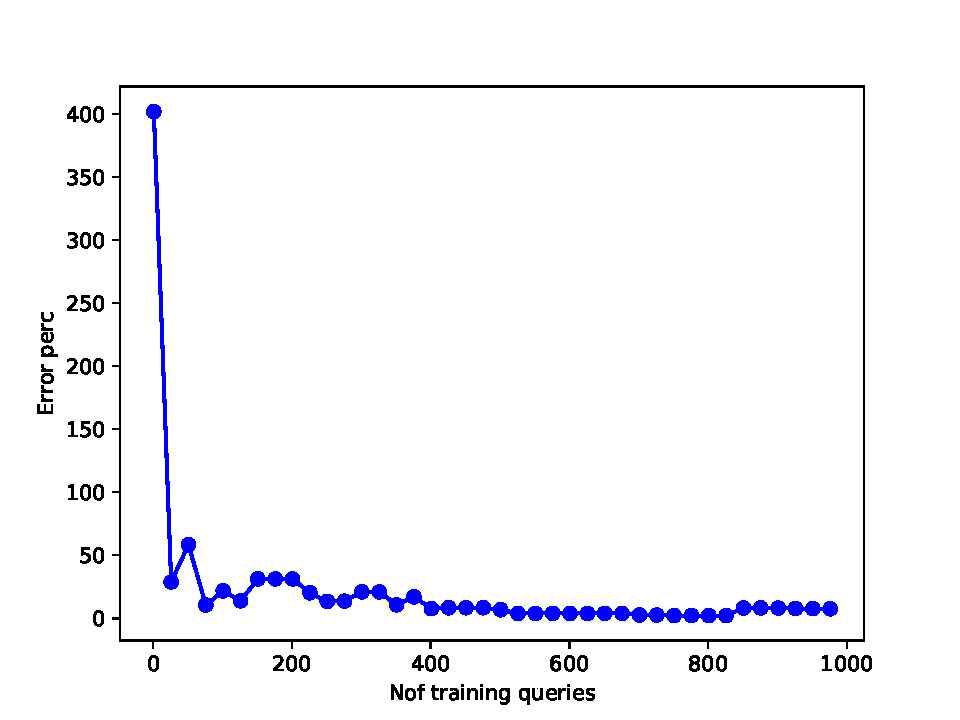
\includegraphics[scale=0.4]{figs/airtraffic/airtraffic_sel11_error.pdf}
   \caption{Query 11 select error}
   \label{fig:sel11}
 \end{subfigure}
 \begin{subfigure}[t]{0.5\textwidth}
   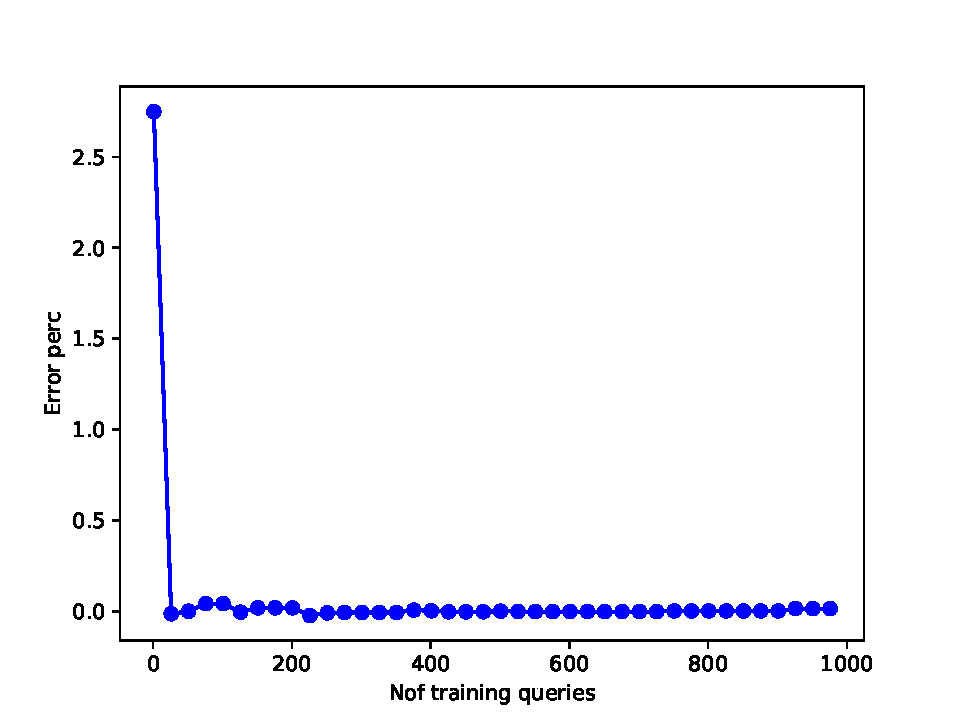
\includegraphics[scale=0.4]{figs/airtraffic/airtraffic_q11_memerror.pdf}
   \caption{Query 11 memory footprint}
   \label{fig:sel11}
  \end{subfigure}


\end{figure}


\subsubsection{Q15}

\begin{figure}[htb!]
\begin{lstlisting}[frame=single]
WITH t1 AS (
    SELECT "Carrier", CAST (FLOOR("CRSDepTime"%2400/100) AS INT) AS "Hour",
           CAST(AVG("ArrDelay") AS DECIMAL(8,2)) AS "PredictedArrDelay"
    FROM ontime
    WHERE Carrier = 'EA'
    GROUP BY "Carrier", "Hour"
),
t2 AS (
    SELECT t."Carrier", tmp.*
    FROM tmp, (SELECT DISTINCT "Carrier" FROM t1) AS t
)
SELECT "Carrier", "Hour", SUM("PredictedArrDelay")
FROM (SELECT * FROM t1 UNION SELECT * FROM t2) AS t
GROUP BY "Carrier", "Hour"
ORDER BY "Carrier", "Hour";
\end{lstlisting}
  \caption{Query 15}
  \label{sel:sql15}
\end{figure}


\begin{figure}[htb!]
  \begin{subfigure}[t]{0.5\textwidth}
    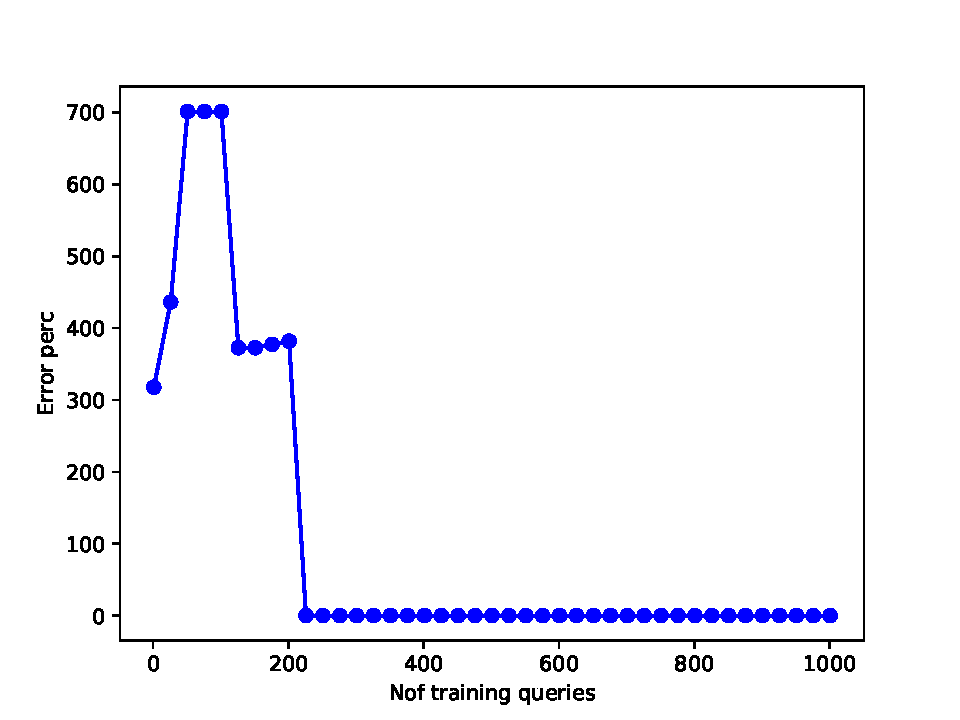
\includegraphics[scale=0.4]{figs/airtraffic/airtraffic_sel15_1_error.pdf}
    \caption{Query 15 select error}
    \label{fig:sel19}
  \end{subfigure}
  \begin{subfigure}[t]{0.5\textwidth}
    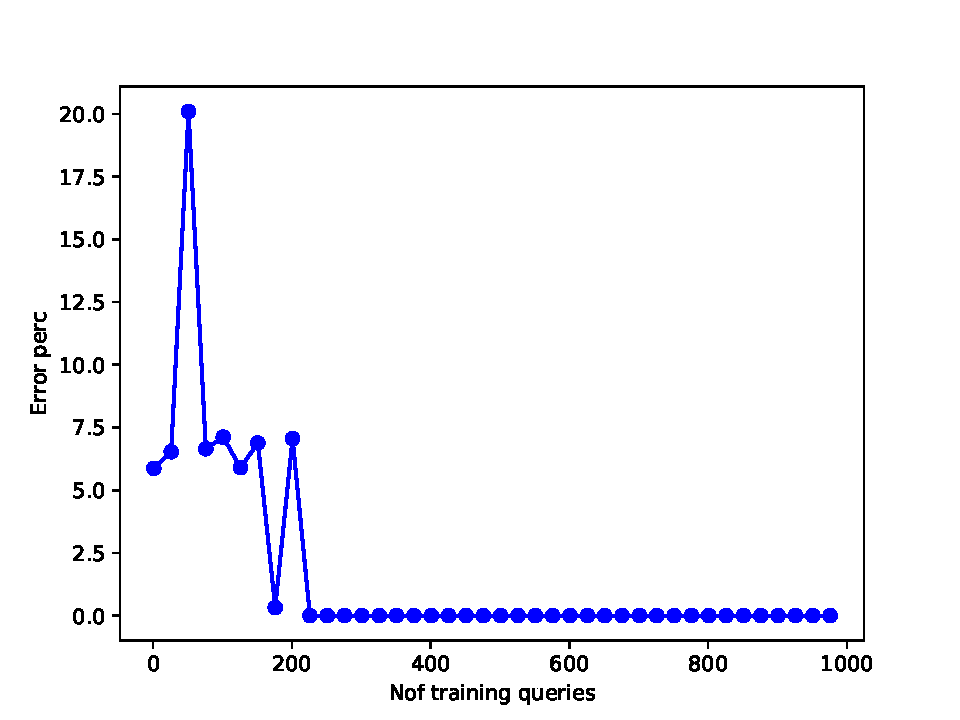
\includegraphics[scale=0.4]{figs/airtraffic/airtraffic_q15_1_memerror.pdf}
    \caption{Query 15 memory footprint}
    \label{fig:sel19}
   \end{subfigure}

\end{figure}

\subsubsection{Q19}

\begin{figure}[htb!]
\begin{lstlisting}[frame=single]
SELECT CAST (FLOOR("CRSDepTime"%2400/100) AS INT) AS "Hour",
       "Origin", "Dest", "Carrier",
       CAST(SUM("DepDel15") AS DOUBLE)/COUNT(*) >= 0.5 AS "PossibleLongDelay"
FROM ontime
WHERE Carrier = 'EV'
GROUP BY "Origin", "Dest", "Carrier", "Hour"
ORDER BY "PossibleLongDelay", "Hour", "Origin", "Dest", "Carrier";
\end{lstlisting}
  \caption{Query 19}
  \label{sel:sql19}
\end{figure}


\begin{figure}[t!]
  \begin{subfigure}[t]{0.5\textwidth}
    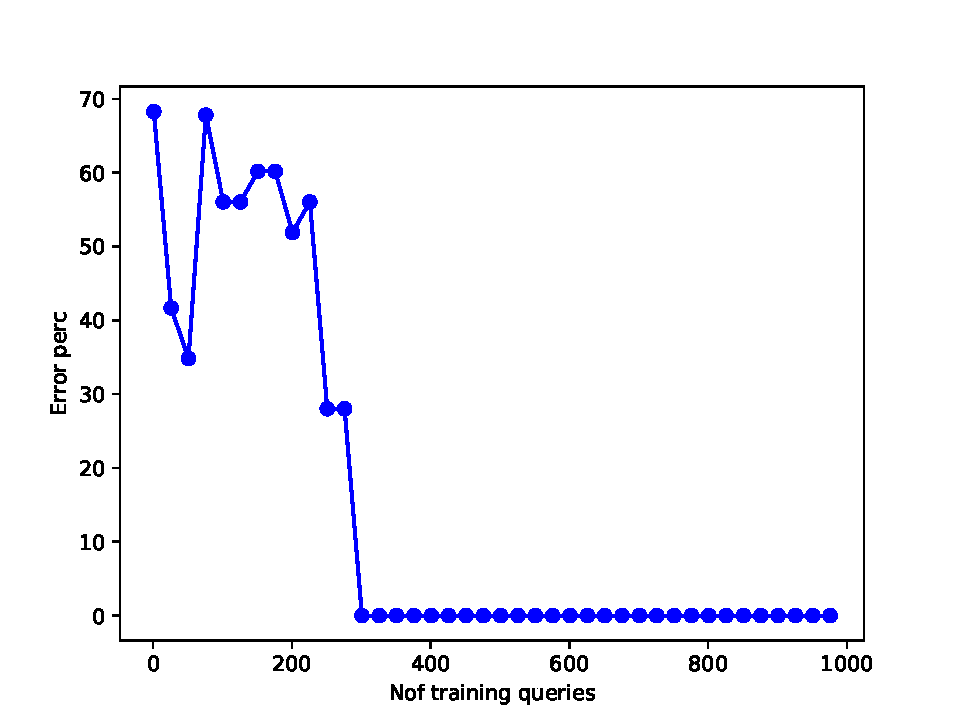
\includegraphics[scale=0.4]{figs/airtraffic/airtraffic_sel19_1_error.pdf}
    \caption{Query 19 select error}
    \label{fig:sel19}
  \end{subfigure}
  \begin{subfigure}[t]{0.5\textwidth}
    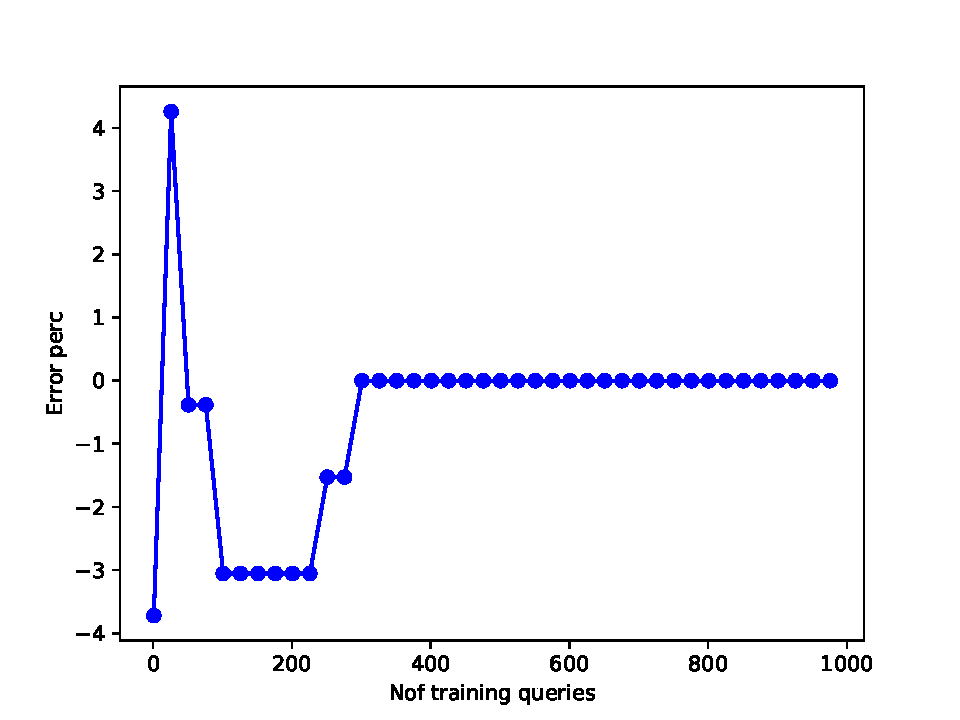
\includegraphics[scale=0.4]{figs/airtraffic/airtraffic_q19_1_memerror.pdf}
    \caption{Query 19 memory footprint}
    \label{fig:sel19}
   \end{subfigure}

\end{figure}



% \begin{figure}[ht]
%   \centering
%   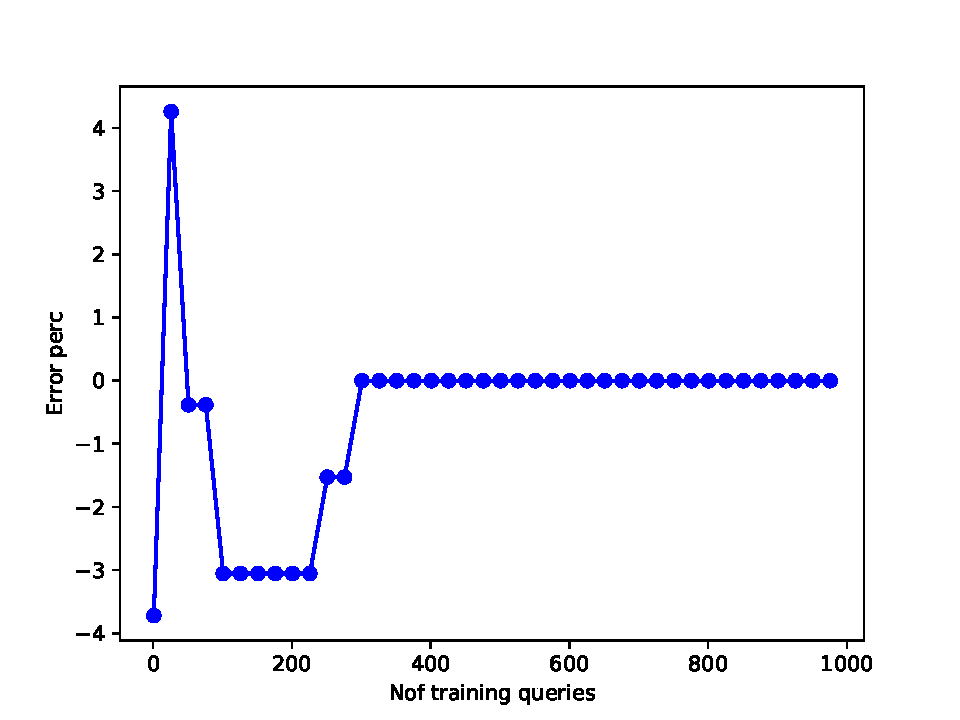
\includegraphics[scale=0.7]{figs/airtraffic/airtraffic_q19_1_memerror.pdf}
%   \caption{Query 4 memory footprint}
%   \label{fig:sel6}
% \end{figure}

%todo list query


\end{document}


\subsection*{Acknowledgments}
This research has received funding from the European Union’s Horizon 2020 research and innovation programme under Grant Agreement no. 732366 (ACTiCLOUD).

{\small
\bibliography{references}
\bibliographystyle{alpha}
}
%\printindex
\subsection*{Appendix}
In this section we collect some user scenarios. screenshots of how it should feel.
and scripts.
